\documentclass{spy}
\course{Time-Domain Astrophysics}
\topic{Variable Stars}

\begin{document}

\tableofcontents

\section{General Comments}
They are found:
\begin{itemize}
    \item across whole range of stellar masses
    \item in many regions of the HRD
    \item in many major phases of stellar evolution
\end{itemize}

They are usually easy to see, as variable.
They provide insights into stellar physics.
They can be used as distance measures, e.g. expansion of Universe, and 3D mapping of SMC, via their period-luminosity relation.


See \url{https://www.aavso.org/}

\section{Classification}
Broad types:
Based on observability:
\begin{itemize}
\item Intrinsic, e.g. due to pulsation, explosion
\item Extrinsic, e.g. eclipsing binaries
\end{itemize}

\begin{figure}[ht]
    \centering
    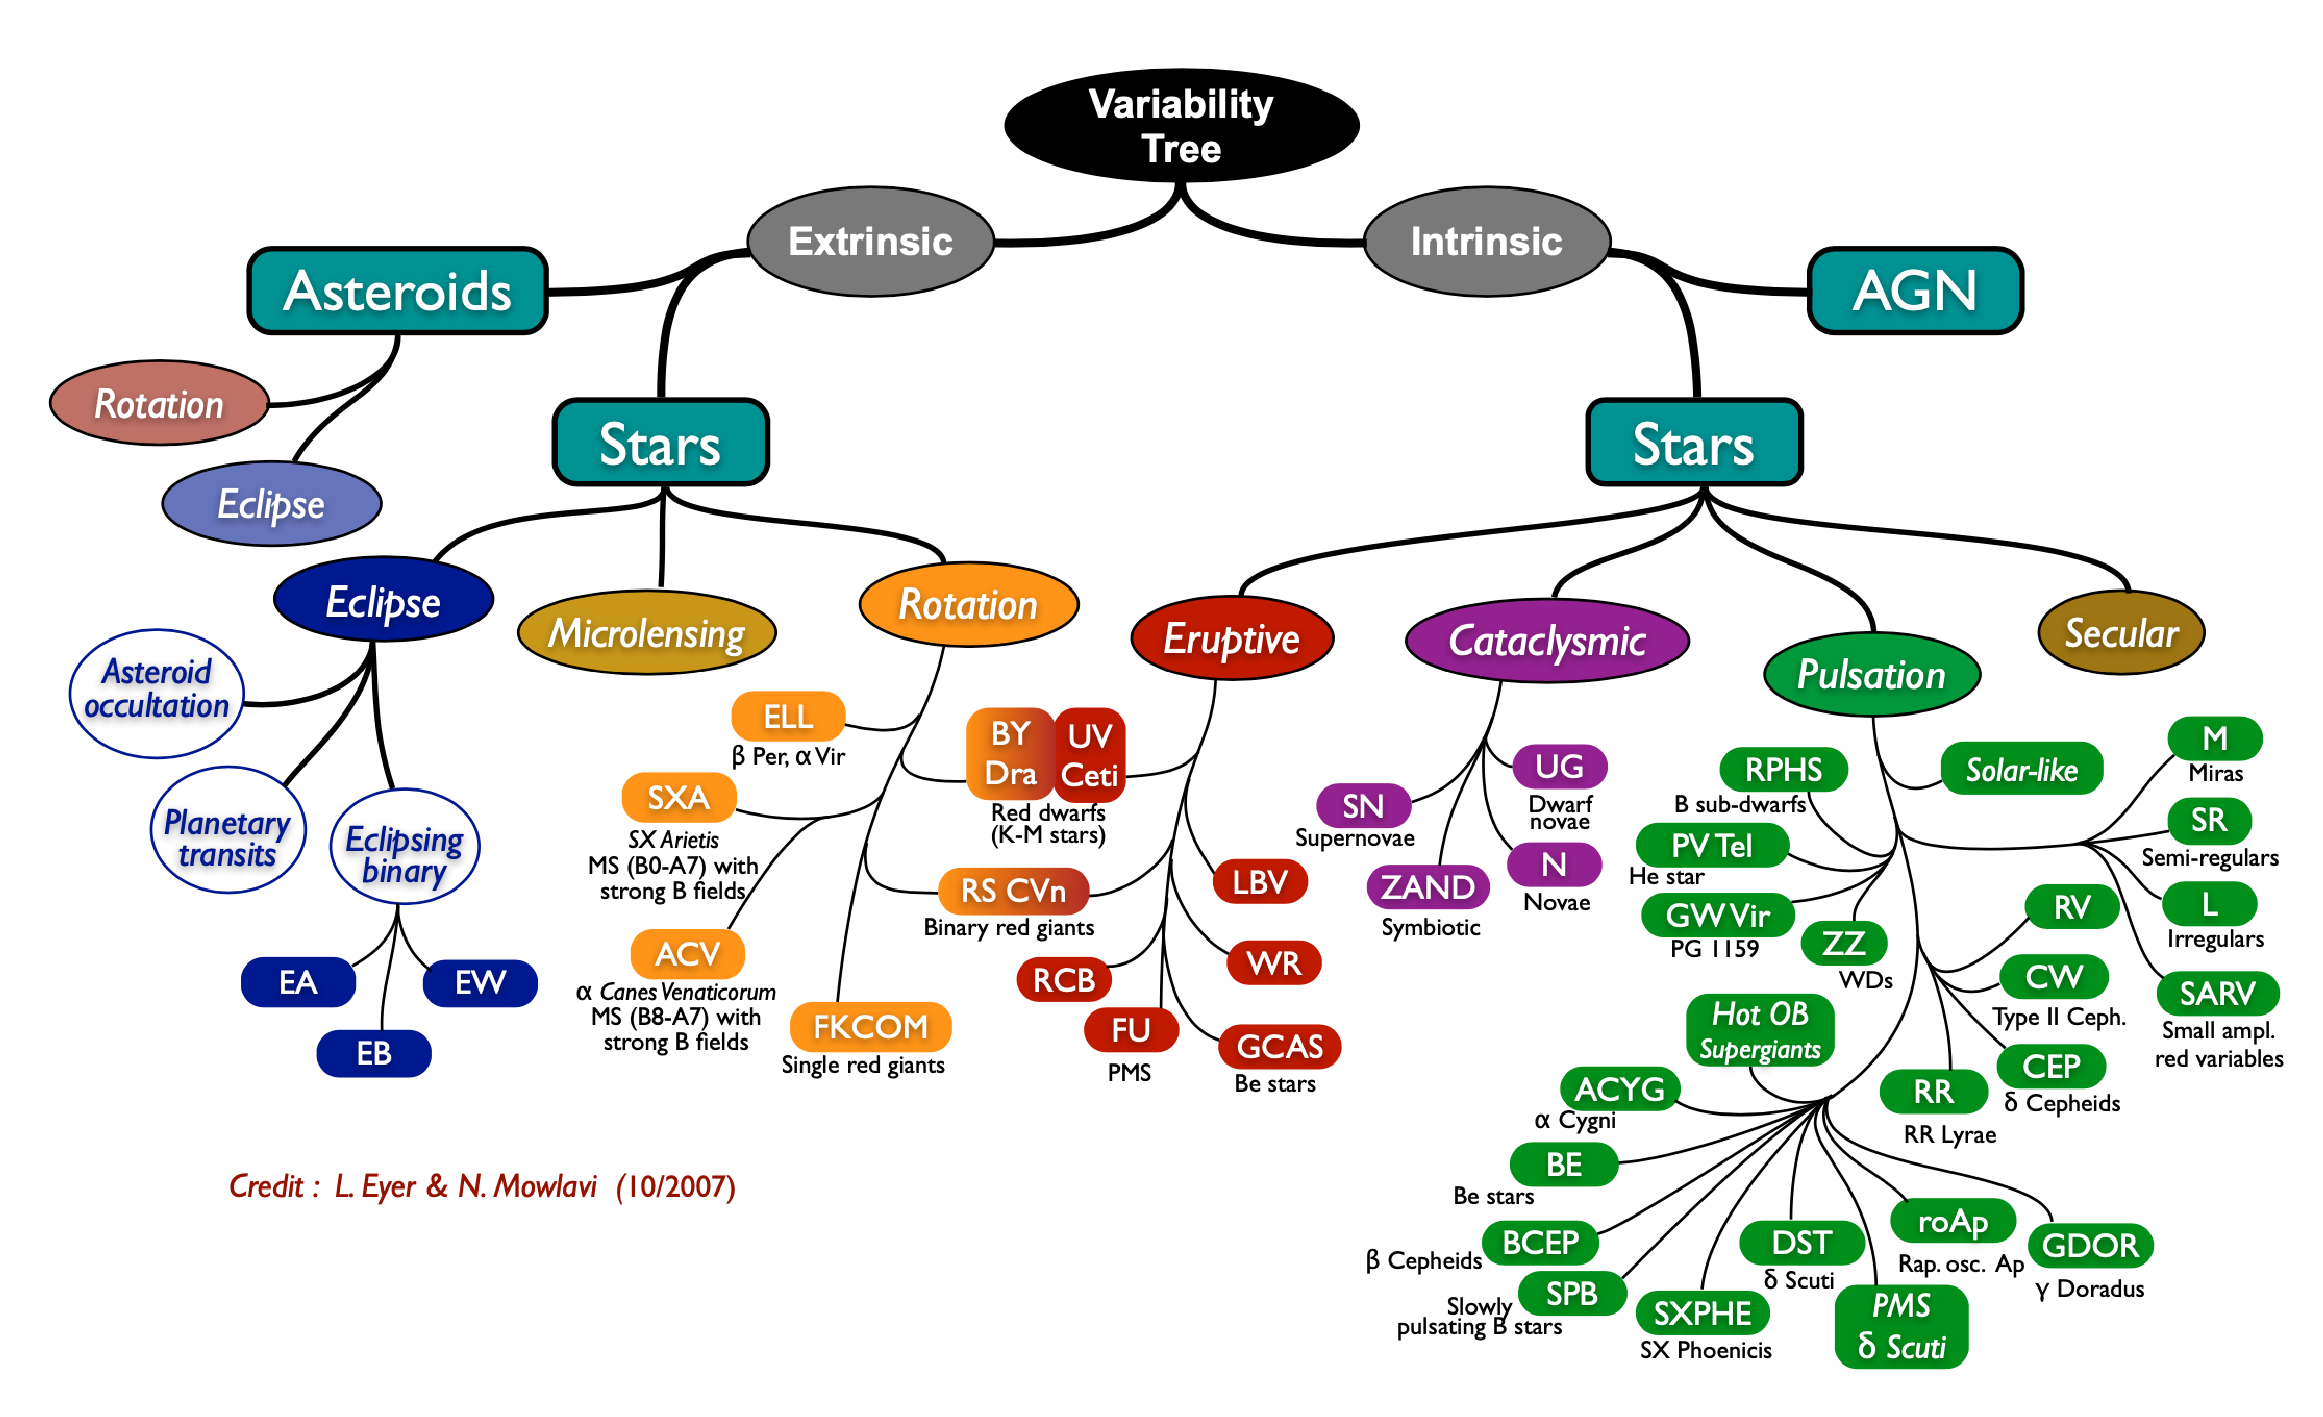
\includegraphics[width=\textwidth]{variable_classes.eps}
    \caption{Classification of Variables. From \citet{eyerVariableStarsObservational2008}}
    \label{variable_classes_diagram}
\end{figure}

Based on observability:
\begin{itemize}
\item Naked-eye (e.g. Mira, Algol, \(\delta\) Cephei)
\item Telescope
\end{itemize}

Based on light-curve features:
\begin{itemize}
\item Period
\item Amplitude (band-dependent)
\item Variability
    \begin{itemize}
    \item Highly regular
    \item Semi-variable
    \item Multi-phase periodic
\end{itemize}\end{itemize}

Based on HRD features:
\begin{itemize}
\item Position on HRD within a group (e.g. WDs, MS, AGB, HB, YSG)
\item Spectral type
\item Luminosity (band-dependent)
\item Colour
\end{itemize}


\section{Physical Factors Influencing Observations}
Factors include:
\begin{itemize}
\item convective zones of star
\item rotation
\item magnetic fields
\item envelope size
\item average density
\item opacity
\item ionisation
\item metallicity/Population
\item energy production
\item extinction, reddening or amplification by circumstellar dust
\item stellar wind and mass loss
\item non-eclipsing binarity or trinarty (or multarity)
\end{itemize}

\section{Period-Density Relation}
Higher AVERAGE density - shorter period. Density signifies evolutionary point of star too. 
e.g. LPVs are giant stars with extended envelopes - low average density, so long period.

WDs compact and dense, hence short period. 


\section{List of Variable Stars and Their Features}
See Table~\ref{variable_stars}.

\begin{figure}[ht]
    \centering
    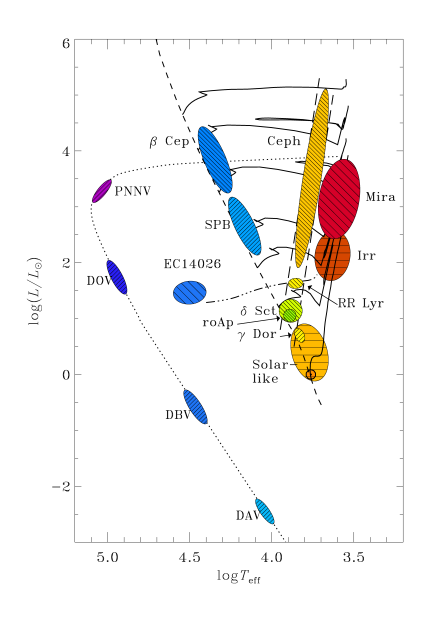
\includegraphics[width=0.8\textwidth]{hrd_variables.eps}
    \caption{Variables on the HRD. From \citet{MiraVariablesPeriod}}
    \label{hrd_variables_diagram}
\end{figure}


\section{Amplitude-Period Relationship}

\begin{figure}[ht]
    \centering
    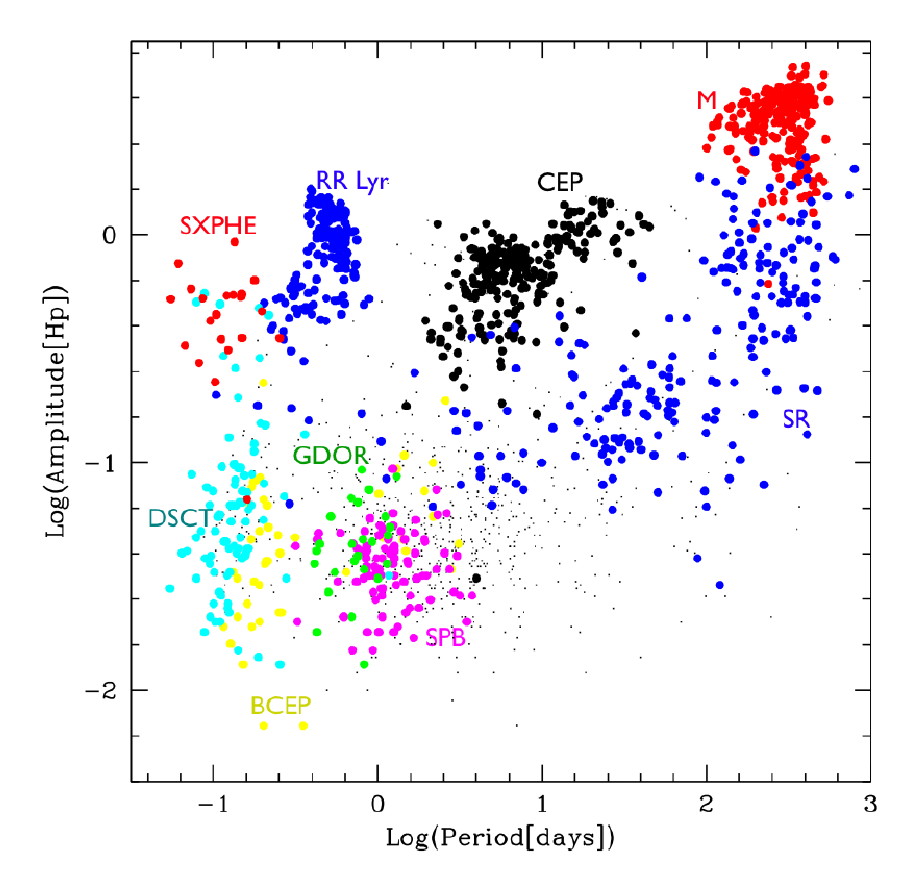
\includegraphics[width=0.8\textwidth]{period_amplitude.eps}
    \caption{Log-Period Log-Amplitude Diagram for Variable Stars. From \citet{eyerVariableStarsObservational2008}}
    \label{period_amp_diagram}
\end{figure}

\section{Spherical Harmonics}
xxx

\section{One-Zone Model}
xxx

\section{Thermodynamics}
\subsection{The '\(\kappa\) Mechanism'}
Radiation flux - opacity (\(\kappa\)) increases with temperature due to partial ionisation (e.g. He\(^+\) to He\(^{++}\) in RR Lyrae and Cepheids), trapping EM radiation/heat, favouring pulsation. 

\subsection{The '\(\epsilon\) Mechanism'}
\begin{equation}
\epsilon \propto T^\nu
\end{equation}

\subsection{The '\(\gamma\) Mechanism'}
Akin to a phase transition (like ice to liquid water). Energy goes in, but temperature doesn't go up (as much as would be expected). 

\section{The Finite Fourier Transform}
\begin{equation}
F_\mathrm{T}(\nu) = \int_{-T/2}^{T/2} f(t)e^{-i 2\pi \nu t} \,dt
\end{equation}

\section{Period-Luminosity (P-L) Relation - the Leavitt Law}

Published by Henrietta Leavitt in 1912 \citep{leavittPeriods25Variable1912}. Figure~\ref{leavitt_period_luminosity_diagram} shows the original figure from the 1912 paper, with log period vs apparent magnitude for the 25 SMC Cepheids.

\begin{figure}[ht]
    \centering
    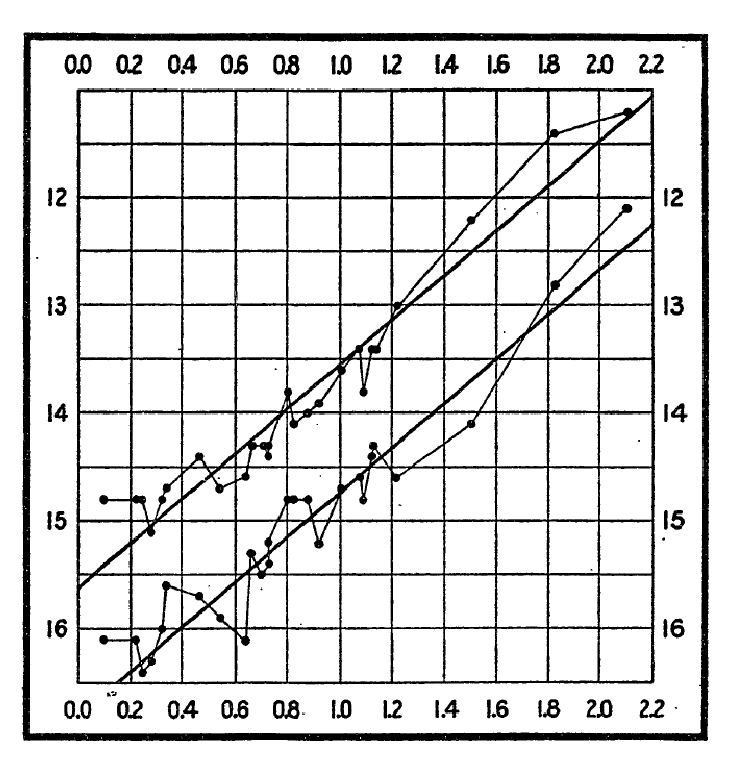
\includegraphics[width=0.6\textwidth]{leavitt_period_luminosity.eps}
    \caption{Log-Period vs Apparent Magnitudes (and their amplitude of change) for 25 Cepheids in the SMC. From \citet{leavittPeriods25Variable1912}}    \label{leavitt_period_luminosity_diagram}
\end{figure}

\subsection{Period-Luminosity-Colour (PLC) Relation}

\subsection{Calibration of the Cepheid PL Relation}
Methods
\begin{itemize}
    \item Parallax
        \begin{itemize}
        \item Direct parallax (Hipparcos satellite)
        \item Gaia
        \end{itemize}
    \item Open cluster main-sequence fitting
    \item Baade-Wesselink method
\end{itemize}

\citet{fouqueNewCalibrationGalactic2007} compared V-band and K-band measurements - K-band was brighter and tighter (Figure~\ref{fouque_cepheid})

\begin{figure}[ht]
    \centering
    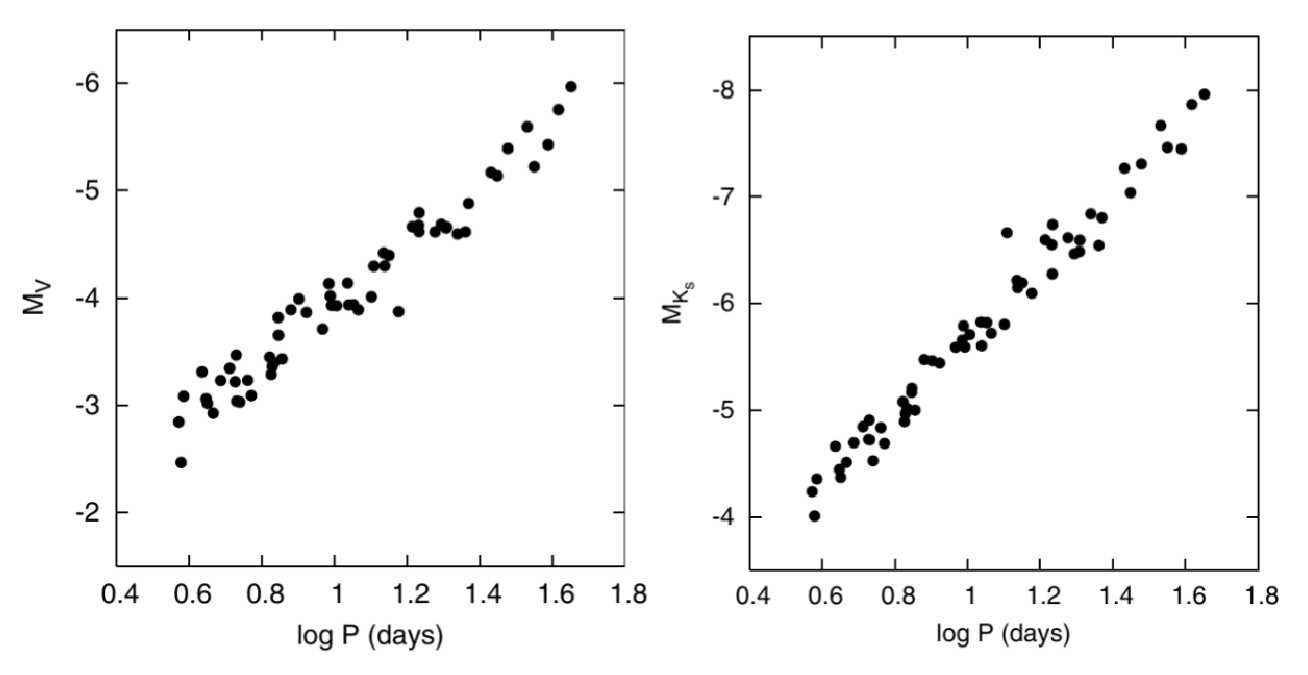
\includegraphics[width=0.7\textwidth]{fouque_cepheid.eps}
    \caption{V-Band vs K-Band calibration of the PL relation for Cepheids in the the Milky Way and LMC. From \citet{fouqueNewCalibrationGalactic2007}}   
    \label{fouque_cepheid}
\end{figure}

The distance modulus:
\begin{equation}
\mu \equiv m-M = 5\log_\mathrm{10}(d) - 5
\end{equation}

Cepheids, primary distance indicators, are exceedingly bright YSGs. Ground-based telescopes can see them a few Mpc away; HST up to 20 Mpc. 

LPVs are a complex zoo of variables - PL relations are varied. 

\section{Baade-Wesselink(-Becker) Method}

Start with:
\begin{equation}
    L = 4 \pi R^2 \sigma T_\mathrm{eff}
\end{equation}
Take logs and multiply by -2.5:
\begin{equation}
    M = a \log_\mathrm{10}(R) + b \log_\mathrm{10}(T_\mathrm{eff})
\end{equation}
Subtract end phase from start phase of pulsation:
\begin{equation}
    M_\mathrm{1}- M_\mathrm{2}= a \log_\mathrm{10}(R_\mathrm{1}/R_\mathrm{2}) + b \log_\mathrm{10}(T_\mathrm{eff,1}/T_\mathrm{eff,2})
\end{equation}
Difference in apparent mags same as difference in absolute mags, so:
\begin{equation}
    \Delta m \equiv m_\mathrm{1}- m_\mathrm{2}= a \log_\mathrm{10}(R_\mathrm{1}/R_\mathrm{2}) + b \log_\mathrm{10}(T_\mathrm{eff,1}/T_\mathrm{eff,2})
\label{baade_1}
\end{equation}
Measure \(m_\mathrm{1}\), \(m_\mathrm{2}\), and \(T_\mathrm{eff}\), then measure radial velocity (\(V_\mathrm{R}\)), the change in radius w.r.t. time:
\begin{equation}
    V_\mathrm{R}(t) = \frac{dR}{dt}
\end{equation}
Therefore:
\begin{equation}
    R = \int V_\mathrm{R}(t) \,dt
\end{equation}
Thus:
\begin{equation}
    R_\mathrm{2} - R_\mathrm{1} = \int_{t_\mathrm{1}}^{t_\mathrm{2}} V_\mathrm{R}(t) \,dt
\label{baade_2}
\end{equation}
Combine Eq.(\ref{baade_1}) and Eq.(\ref{baade_2}) to give 2 equations with 2 unknowns, and can then solve for \(R_\mathrm{1}\) and \(R_\mathrm{2}\).
Repeat multiple times over whole pulsation cycle, to get average radius.
Nowadays interferometry can be used to measure radius. 


\bibliographystyle{mnras}
\bibliography{variables_bibliography}

\end{document}
